
\begin{enumerate}
    \item A block of mass \(2M\) is attached to a massless spring with spring-constant \(k\). This block is connected to two other blocks of masses \(M\) and \(2M\) using two massless pulleys and strings. The accelerations of the blocks are \(a_1\), \(a_2\) and \(a_3\) as shown in the figure. The system is released from rest with the spring in its unstretched state. The maximum extension of the spring is \(x_0\). Which of the following option(s) is/are correct? [\(g\) is the acceleration due to gravity. Neglect friction]
        \begin{tasks}(2)
            \task \(x_0 = \frac{4Mg}{k}\)
            \task When spring achieves an extension of \(\frac{x_0}{2}\) for the first time, the speed of the block connected to the spring is \(3g\sqrt{\frac{M}{5k}}\)
            \task At an extension of \(\frac{x_0}{4}\) of the spring, the magnitude of acceleration of the block connected to the spring is \(\frac{3g}{10}\)
            \task \(a_2 - a_1 = a_1 - a_3\)
        \end{tasks}
\end{enumerate}
\begin{center}
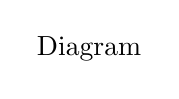
\begin{tikzpicture}
\node {Diagram};
\end{tikzpicture}
\end{center}
